% =====================================================================
%  第 6 章 §6.6 中段 —— ch06e（tr05）
%  页段：PDF 363–372（原书 p.353–362）
%  本块不是章首也不是节首：直接续写正文，不写 \chapter / \section
% =====================================================================

% [原文 p.353]
设 $\psi$ 为完全辛同胚，则由定理 6.215 与“定理 6.129”，确定双射 $\psi_*:\cM(L)\to\cM(\psi(L))$。又，对横截的拉格朗日子流形组 $L_1,L_2$ 与 $p\in L_1\cap L_2$，确定 Maslov–Viterbo 指数（Maslov index）$\mu(p)$（参看 [290]）。

\begin{theorem}{6.226}
  设 $L_1,L_2$ 为拉格朗日子流形，$b_i\in\cM(L_i)$。Floer 同调 $HF((L_1,b_1),(L_2,b_2))$ 作为有限生成 $\Lambda_{\mathrm{nov},+,\Q}$ 模而确定，并具有下列性质。
  (1) 当 $L_1=L_2=L$，$b_1=b_2=b$ 时，它与定义 6.221 的 $HF((L,b),(L,b))$ 作系数扩张到 $\Lambda_{\mathrm{nov},+,\Q}$ 所得者一致。
  (2) 设 $L_1$ 与 $L_2$ 横截，$L_1\cap L_2=\{p_1,\dots,p_N\}$。以 $[p_i]$ 为次数 $\mu(p_i)$ 的生成元的自由 $\Lambda_{\mathrm{nov},+,\Q}$ 模上确定边界算子，$HF((L_1,b_1),(L_2,b_2))$ 与该边界算子的上同调一致。
  (3) 设 $\psi_i$ 为完全辛同胚，则 $HF((L_1,b_1),(L_2,b_2))$ 与 $HF((\psi_1(L_1),\psi_{1*}(b_1)),(\psi_2(L_2),\psi_{2*}(b_2)))$ 之间存在标准的同构。
\end{theorem}

\begin{remark}{6.227}
  定理 6.226 的 Floer 同调随 $b_1,b_2$ 的取法而变，并不只由拉格朗日子流形决定。发生这种情况的原因是模空间 $CM_{0,k}(M,J_M;L;\beta)$ 带边界。这与 Donaldson 在 [74] 中对 $b_2^+=1$\footnote{指 $H^2(M;\Q)$ 的相交形式的正特征值为 1。} 的 4 维流形的 Donaldson 不变量所发现的、称为跨墙（wall crossing）的现象，本质上有相同的理由。这称为 Floer 同调的跨墙。$b_2^+=1$ 的 4 维流形的 Donaldson 不变量用（不定 2 次形式的）theta 函数表示（Göttsche–Zagier [170]、Borcherds [47]、Moore–Witten [261]）。如后面所见，拉格朗日子流形的 Floer 同调中也出现（不定 2 次形式的）theta 函数。（不定 2 次形式的）theta 函数之所以出现，是因为两者都是跨墙。
\end{remark}

回到与镜像对称的关系的说明。下述猜想是 6.83 的类似。

\begin{conjecture}{6.228}
  把几何链看作流（current）。(6.70) 对充分接近 0 的正数 $T$ 作为流收敛。
\end{conjecture}

% [原文 p.354]
\begin{remark}{6.229}
  (6.70) 中取的是无限和，因此若把数代入 $T$，就不能在几何链的范畴内完成讨论。扩大到流则可以，但会产生与流的拉回有关的困难（参看注 5.80）。用形式幂级数与几何链讨论，在最后一刻把数代入 $T$，就能回避这个困难。[121] 中对 $M$ 为辛环面的情形，就若干个拉格朗日子流形证明了猜想 6.228，并实行了用流的构造，那里用的就是这一方法。
\end{remark}

以下暂时假定猜想 6.228。与猜想 6.83 一样，改写为形式幂级数的语言，大概可以回避猜想的某些部分；但必须在取同调之前的链的层面讨论，故改写比猜想 6.83 的情形更困难\footnote{笔者认为，猜想 6.228 的证明大概是同调镜像对称的证明中遗留的最困难的一点之一。}。把 $T$ 换成 $T^C$，相当于把 $\omega$ 换成 $C\omega$。因此，考虑大体积极限，就可与 §6.3 一样取 $T=e^{-1}$。

至今暂时只考虑拉格朗日子流形，而忽略了其上的复线丛。就这一点作简单说明。有 $B$ 场时也同样可以，但为简单起见这里设 $B$ 场为 0。

设 $\mathfrak{L}\to L$ 为平坦 $U(1)$ 丛。设 $\beta\in\pi_2(M)$，则确定 $\partial\beta\in\pi_1(L)$。以 $\operatorname{hol}_{\mathfrak{L}}(\beta)$ 表示 $\mathfrak{L}$ 沿 $\partial\beta$ 的和乐（$\in U(1)$）。于是，把 (6.70) 换成下式，就定义了考虑 $\mathfrak{L}$ 时的弱 $A_{\infty}$ 代数。
\begin{equation}
  \mathrm{m}_k=\sum\mathrm{m}_{k,\beta}\operatorname{hol}(\beta)\exp(-\beta\cap\omega)u^{\mu(\beta)/2}. \tag{6.73}
\end{equation}
右边看作 $\C[u,u^{-1}]$ 系数的流。若假定猜想 6.228，则 (6.73) 定义弱 $A_{\infty}$ 代数。于是形变的模空间 $\cM(L;\mathfrak{L})$ 作为复解析空间（complex variety）而确定。另一方面，对 $\cM(L;\mathfrak{L})$ 的每个元 $b$，确定（收敛幂级数版的）$A_{\infty}$ 代数 $(\mathit{IIC}(L,\mathfrak{L};\C[u,u^{-1}]),\mathrm{m}^b_*)$。

考虑 $B$ 模型。设 $\cF$ 为解析凝聚层。

% [原文 p.355]
\begin{equation}
  \cF\to\cF_1\to\cdots \tag{6.74}
\end{equation}
为内射分解（injective resolution）。（$\cF$ 为正则向量丛时，用 $\cF$ 系数的 Dolbeault 复形也可以。）

置
\[
  C(\cF,\cF)=\bigoplus_{i,j}\operatorname{Hom}(\cF_i,\cF_j),
\]
把 $C(\cF,\cF)$ 上的算子 $\mathrm{m}_1$ 取为由 (6.71) 确定的微分，$\mathrm{m}_2$ 取为由合成确定的积。

由于 $(C(\cF,\cF),\mathrm{m}_1,\mathrm{m}_2)$ 是微分代数，置 $\mathrm{m}_3=\cdots=0$，并按 (6.34) 之后所述移动符号，就确定 $A_{\infty}$ 代数 $(\mathit{IIC}(\cF,\cF),\mathrm{m}_1,\mathrm{m}_2)$。
% [Tutor Note: 原书把这一族 $A_{\infty}$ 代数写作 $\mathit{IIC}(\cdots)$，字形是两条竖线加 C（不是 $HC$）；正文照录，全书统一作 $\mathit{IIC}$。它与前面的 $\mathrm{HC}$ 系记号无关。]

\begin{conjecture}{6.230}
  对 $b\in\cM(L;\mathfrak{L})$，确定 $\cF_{L,\mathfrak{L},b}$，且 $A_{\infty}$ 代数 $(\mathit{IIC}(L,\mathfrak{L};\C[u,u^{-1}]),\mathrm{m}^b_*)$ 与 $(C(\cF_{L,\mathfrak{L},b},\cF_{L,\mathfrak{L},b}),\mathrm{m}_1,\mathrm{m}_2)\otimes\C[u,u^{-1}]$ 同伦等价。
\end{conjecture}

猜想 6.230 是包含 Frobenius 代数的一致性的、更精细的同调镜像对称猜想的表述。进而，用定理 6.226 的 Floer 同调的收敛幂级数版，可以预期
\begin{equation}
  \operatorname{Ext}(\cF_{L_1,\mathfrak{L}_1,b_1},\cF_{L_2,\mathfrak{L}_2,b_2})\cong HF((L_1,\mathfrak{L}_1,b_1),(L_2,\mathfrak{L}_2,b_2)) \tag{6.75}
\end{equation}
\footnote{有平坦丛时 Floer 同调的定义，例如参看 [116]、[121]。}\footnote{用收敛幂级数考虑的 Floer 同调，若不把 1 圈（loop）的贡献（即注 5.48 提到的、含 Hutchings 不变量量子效应的类似物）计入，就不成为正确的定义。这一点预定在 [125] 中叙述。}。(6.75) 的同构与积结构相容，这是下一个猜想。也就是说，猜想下图式 (6.76) 可交换。

这里进入第 1 行的积结构是 Massey–Yoneda 积，第 2 行的映射是笔者的 [114] 中（推广 Donaldson 的想法 [76] 而）引入的、用 Floer 同调在 $A_{\infty}$ 范畴中的态的合成。

% [原文 p.356]
\begin{equation}
  \resizebox{0.97\linewidth}{!}{$\displaystyle \begin{array}{ccc} \operatorname{Ext}(\cF_{L_1,\mathfrak{L}_1,b_1},\cF_{L_2,\mathfrak{L}_2,b_2}) \otimes\operatorname{Ext}(\cF_{L_2,\mathfrak{L}_2,b_2},\cF_{L_3,\mathfrak{L}_3,b_3}) & \longrightarrow & \operatorname{Ext}(\cF_{L_1,\mathfrak{L}_1,b_1},\cF_{L_3,\mathfrak{L}_3,b_3})\\[2mm] \big\downarrow{\scriptstyle\cong} & & \big\downarrow{\scriptstyle\cong}\\[2mm] HF((L_1,\mathfrak{L}_1,b_1),(L_2,\mathfrak{L}_2,b_2)) \otimes HF((L_2,\mathfrak{L}_2,b_2),(L_3,\mathfrak{L}_3,b_3)) & \longrightarrow & HF((L_1,\mathfrak{L}_1,b_1),(L_3,\mathfrak{L}_3,b_3)) \end{array} $} \tag{6.76}
\end{equation}
% [Tutor Note: 图式 (6.76) 的纵向两个箭头都是 (6.75) 的同构 $\cong$；横向箭头是两个复合：上行是 Ext 的合成（即正文所说的 Massey–Yoneda 积），下行是 Floer 同调中态的合成。原书方形图中央还有一个表示“图式可交换”的圆弧记号，用 array 排版时不重现。]

\begin{remark}{6.231}
  笔者的论文 [114] 中有与观察 6.206(1) 有关的错误。这一点在拉格朗日子流形单调且 Maslov 指数为 3 以上的情形，已在 [119] 中订正。（Oh [290] 证明观察 6.206(1) 不发生，正是这种情形。）由定理 6.215、定理 6.226，对这一问题点的理解已充分完成，因此对一般的辛流形，作 $A_{\infty}$ 范畴的准备已经就绪；但其细节尚未写出。所以本书关于拉格朗日子流形所成的 $A_{\infty}$ 范畴，不再多述。
\end{remark}

\begin{remark}{6.232}
  由猜想 6.230（即 (6.75) 中 $(L_1,\mathfrak{L}_1,b_1)=(L_2,\mathfrak{L}_2,b_2)$ 的情形），前面保留未说明的“点层的镜像应为拉格朗日环面”这一事实可如下说明。即，对点层 $\cF_p$ 有环同构
  \[
    \operatorname{Ext}^*(\cF_p,\cF_p)\cong H^*(T^n;\C)
  \]
  （参看 [280] 等）。因此，$\cF_p$ 的镜像即拉格朗日子流形 $L$，必须满足 $HF(L,L)\cong H^*(T^3;\C)$。这提示 $L\cong T^3$。

  另外，三维 Calabi–Yau 流形 $M^\dagger$ 若满足 $H^1(M^\dagger;\Q)=0$，则结构层 $\cO_{M^\dagger}$ 满足 $\operatorname{Ext}^*(\cO_{M^\dagger},\cO_{M^\dagger})\cong H^{0,*}(M^\dagger;\C)$，故其镜像即拉格朗日子流形大概应是有理同调 3 球面。（不过 $L$ 的 Floer 上同调与 $L$ 的普通上同调未必一致，故不必 $H^*(L;\Q)\cong H^*(S^3;\Q)$，只须 $HF^*(L,L)\cong H^*(S^3;\Q)$ 即可。）
\end{remark}

\begin{remark}{6.233}
  在 (6.74) 中考虑 $\cF_{L_1,\mathfrak{L}_1,b_1}=\cF_{L(p),\mathfrak{L}(p),b(p)}$ 为点层 $\cF_p$、$\cF_{L_2,\mathfrak{L}_2,b_2}=\cF_{L,\mathfrak{L},b}$ 为正则向量丛 $\mathfrak{E}$ 的情形。此时
  \[
    HF^n((L(p),\mathfrak{L}(p),b(p)),(L,\mathfrak{L},b))\cong\operatorname{Ext}^n(\cF_p,\mathfrak{E})\cong\mathfrak{E}_p
  \]
  （$\mathfrak{E}_p$ 是 $\mathfrak{E}$ 在 $p$ 处的纤维）。因此，有可能把 $\mathfrak{E}$ 作为“移动拉格朗日子流形时 Floer 同调的族”来构造。
\end{remark}
% [Tutor Note: 这里“点层”指点的结构层 $\cF_p$；$n$ 与 $3$ 的差别来自：一般地 $\operatorname{Ext}^*(\cF_p,\cF_p)\cong H^*(T^n;\C)$，而在 $T^4$ 的镜像理论里点层对应的拉格朗日环面是 3 维的，故下文比较 $H^*(T^3;\C)$。]

% [原文 p.357]
（这个想法基于与 Kontsevich 的讨论（1997 年夏）。）[121] 中对辛环面上的仿射拉格朗日子流形的情形实行了这一点（实例稍后叙述）。要在更一般的情形实行，还有若干困难。猜想 6.228 的证明、$\mathcal{LAG}_{st}(M)$ 的紧化等，是其最困难之处。

同调镜像对称猜想，其猜想的内容本身就多得惊人。可以说，在镜像对称中，辛流形 $M$ 所具有的一切性质都用复流形 $M^\dagger$ 的性质来转述，这被作为猜想提出来。按本章开头所述的镜像对称的想法，即“我们居住的空间的‘内部空间’究竟是 $M$ 还是 $M^\dagger$，没有方法区分”，本来就应当如此。存在某种既非辛流形也非复流形的新的“空间”概念，从它出发，作为其表现方法，辛流形与复流形都能显现出来——这是理想的形式，超弦理论似乎正以此为目标。

同调镜像对称猜想的含义还有很多，但这里不再多述。

下面叙述本节所述的构造与拉格朗日子流形的 Floer 上同调的例子。以下例子把 [121] 与 [122] 合起来即可得到。这些例子中猜想 6.228 可以验证，故用收敛幂级数讨论。考虑复环面 $T^4=\C^2/(\Z[\sqrt{-1}])^2$。设 $z_i=x_i+\sqrt{-1}y_i$ 为 $\C^2$ 的坐标。以 $(z_1,z_2)\mapsto(x_1,x_2,y_1,y_2)$ 把 $\C^2$ 与 $\R^4$ 等同。设 $A=(a^{ij}:i,j=1,2)$、$(b^{ij}:i,j=1,2)$ 为实 $2\times2$ 矩阵，且 $A+A^t$ 正定。置
\[
  \omega_A=\sum a^{ij}dx_i\wedge dy_j,\qquad B=\sum b^{ij}dx_i\wedge dy_j,
\]
则 $\omega_A$ 成为 $T^4$ 与 $\C^2$ 上的辛形式，而 $T^4$ 与 $\C^2$ 上的复结构关于 $\omega_A$ 温和。置 $\tilde\omega_{A,B}=\omega_A+2\pi\sqrt{-1}B$。

依次用 $x_1=x_2=0$、$y_1=y_2=0$、$x_1-y_1=x_2-y_2=0$ 定义 $\C^2$ 的线性子空间 $\tilde L_{pt},\tilde L_{st},\tilde L_{pol}$。容易看出在 $\tilde L_{pt},\tilde L_{st}$ 上 $\omega_A=0$。$A$ 为

% [原文 p.358]
对称矩阵时，$\tilde L_{pol}$ 上也有 $\omega_A=0$，且 $\omega_A$ 成为凯勒形式。

对 $v\in\C^2/\tilde L_{pt}$，以 $\tilde L_{pt}(v)\subset\C^2$ 表示把 $\tilde L_{pt}$ 沿 $v$ 平移所得的仿射拉格朗日子流形。把 $\tilde L_{pt}(v)$ 在 $T^4$ 中确定的拉格朗日子流形（环面）记作 $L_{pt}(v)$。把 $\tilde L_{st},\tilde L_{pol}$ 在 $T^4$ 中确定的拉格朗日子流形写作 $L_{st},L_{pol}$。

设 $\alpha\in\tilde L^*_{pt}$（$*$ 表示作为 $\R$ 向量空间的对偶）。$\alpha$ 可看作 $\tilde L_{pt}$ 上的闭微分 1 形式。由此确定 $L_{pt}(v)$ 上（平凡丛的）平坦 $U(1)$ 联络 $\nabla^\alpha$。
\[
  \mathcal{LAG}_{pt}=\{(L_{pt}(v),\nabla^\alpha)\mid v\in\C^2/\tilde L_{pt},\ \alpha\in\tilde L^*_{pt}\}
\]
是 $\mathcal{LAG}_{st}(T^4,\tilde\omega_{A,B})$ 的连通分支（也是 $\mathcal{LAG}_{sp}(T^4,\tilde\omega_{A,B})$ 的连通分支）。先计算 $\mathcal{LAG}_{pt}$ 上的经典复结构。设 $\alpha=\xi_1dy_1+\xi_2dy_2$，$v=(v_1,v_2)$。映射 $(L_{pt}(v),\nabla^\alpha)\mapsto(v_1,v_2,\xi_1,\xi_2)$ 是从 $\mathcal{LAG}_{pt}$ 的万有覆盖空间到 $\R^4$ 的微分同胚。把 $(v_1,v_2,\xi_1,\xi_2)$ 看作 $\mathcal{LAG}_{pt}$ 的坐标。

\begin{lemma}{6.234}
  关于由 $\tilde\omega_{A,B}$ 确定的 $\mathcal{LAG}_{pt}$ 上的复结构，
  \begin{align*}
    h(v_1,v_2,\xi_1,\xi_2)=\bigl(&(a^{11}v_1+a^{12}v_2)+2\pi\sqrt{-1}(\xi_1+b^{11}v_1+b^{12}v_2),\\
    &(a^{21}v_1+a^{22}v_2)+2\pi\sqrt{-1}(\xi_2+b^{21}v_1+b^{22}v_2)\bigr)
  \end{align*}
  是双全纯映射。
\end{lemma}

证明是简单的计算，故省略。由引理 6.234，$\mathcal{LAG}_{pt}$ 上的复结构已算出。

干脆把猜想 6.193 当作定义。也就是说，

\begin{definition}{6.235}
  把在 $\mathcal{LAG}_{pt}$ 上赋予引理 6.234 的复结构所得的复环面，定义为辛环面 $(T^4,\tilde\omega_{A,B})$ 的镜像，写作 $(T^4,J_{A,B})$。
\end{definition}

\begin{remark}{6.236}
  给 $\mathcal{LAG}_{pt}$ 赋予的是经典复结构，此时不存在量子修正。因为 $\pi_2(T^4;L_{pt})=0$，不存在以 $L_{pt}(v)$ 为边界的伪全纯圆盘；这正是量子修正不存在的理由。
\end{remark}

\begin{remark}{6.237}
  在定义 6.235 中确定镜像时，先指定了属于哪个同调类的拉格朗日子流形在镜像中成为点层。这种取法

% [原文 p.359]
  一变（例如把 $\tilde L_{st}$ 与 $\tilde L_{pt}$ 交换），就得到不同的镜像。这样镜像并不唯一。设 $T^4$ 的两种镜像为 $T^4_1,T^4_2$，则 $T^4_1$ 与 $T^4_2$ 上解析凝聚层范畴的导出范畴互相同构。同构由 Fourier–Mukai 变换（[266]，[267]）给出。在辛环面一侧考虑，应当成为点层的镜像的拉格朗日环面的交换，是由辛同胚导出的“经典”同构。另一方面，在复环面一侧，导出范畴的同构不能由全纯同构导出。这种不同类型的自同构在双对性（此处为镜像对称）下互换的现象，称为双对性的双对性（duality of duality）。
\end{remark}

\begin{remark}{6.238}
  定义 6.235 并非对 $T^4$ 上所有仿射辛结构都确定了其镜像。$T^4$ 的辛结构（＋$B$ 场）的模空间维数为 $\rank H^2(T^4;\C)=6$，而 $(A,B)$ 构成复 4 维的族。$\rank H^{1,1}(T^4;\C)=4$。也就是说，$\tilde\omega_{A,B}$ 的模空间成为（复化）凯勒形式的模空间。（若 $A$ 不对称，则 $\omega_A$ 不是关于 $T^4$ 的标准复结构的凯勒形式；但换一个复结构，它就成为凯勒形式。）在剩下的 2 个维数方向，即 $H^{2,0}(T^4)\oplus H^{0,2}(T^4)$ 方向上移动辛形式，就不再有表示与 $L_{pt}$ 或 $L_{st}$ 相同同调类的拉格朗日环面。换言之，几乎所有情形下 $T^4$ 都不成为拉格朗日纤维丛。此时替代地存在遍历的拉格朗日叶状结构（Lagrange foliation）。用拉格朗日叶状结构的叶空间（＋联络的模空间的对应部分）即非交换环面取代 $\mathcal{LAG}_{pt}$，这个非交换环面就被认为是镜像。[120] 中称之为非交换镜像对称（noncommutative mirror symmetry）。

  用 $B$ 模型考虑，则向 $H^{1,1}(M)$ 以外的方向的辛形式（＋$B$ 场）的形变，应当对应于向 $H^1_{\bar\partial}(M^\dagger;T^{1,0}M)$ 以外的方向的 $M^\dagger$ 的复结构形变，即 §6.5 所述的 Calabi–Yau 流形的扩充形变空间的元素。对环面的情形，如上所述，可对扩充形变空间的某些元素给出基于非交换几何的意义。这种可用拉格朗日叶状结构描述的情形是否还有别的，尚不清楚。以上参看 [120]。
\end{remark}

% [原文 p.360]
\begin{lemma}{6.239}
  若 $A,B$ 为对称矩阵，则镜像 $(T^4,J_{A,B})$ 是阿贝尔簇。
\end{lemma}

本引理的证明，在现阶段直接计算也可作出，但后面会自然明白，故这里不做。复 2 维阿贝尔簇的模空间的复维数为 3。这与对称实矩阵组 $A,B$ 的集合的维数一致。

以下假定 $A,B$ 对称。此时，$T^4$ 上除 $L_{pt}(v)$ 外还有 2 个拉格朗日子流形 $L_{st},L_{pol}$。$L_{st}$ 在同调镜像对称中对应于结构层。$L_{pol}$ 成为 $(T^4,J_{A,B})$ 上的丰富（ample）线丛，并确定极化（polarization）\footnote{这些代数几何术语在以后的构造中未必需要，故不作解说。不知道的话跳过即可。}。（更准确地说，要定义使上述成立的函子“$(T^4,\omega_A)$ 的拉格朗日子流形 $\mapsto$ 解析凝聚层”。其构造本书不叙述。参看 [121]。）

$L_{st}$ 与 $L_{pol}$ 交于 1 点。在该点施行拉格朗日手术（引理 4.145）所得的拉格朗日子流形记作 $L$。此后一段的目标是计算 $HF(L,L_{pt}(v,\nabla^\alpha))$。

在这之前需要一点注意。即拉格朗日手术并不唯一。下面叙述所考察的 $L$ 的情形的取法。在 3 维以上，拉格朗日手术有 2 种，对应于确定引理 4.144 之前出现的函数 $f_\epsilon$ 时出现的数 $\epsilon$ 的符号。只有复 2 维的情形情况不同。（只有在 2 维情形，拉格朗日手术使 $H^1(L;\Q)$ 的秩增加，并产生相应的参数。）在 2 维，拉格朗日手术的方式在定义 6.195 的等价类的意义下与 $S^1$ 的元素对应\footnote{为懂得椭圆曲面（elliptic surface）理论的读者写下：这与 I 型奇异纤维附近的非奇异纤维的复结构模空间有关。}。$L$ 是亏格 2 的曲面。又 $\pi_2(T^4;L)\cong\Z$，其生成元是张在手术所做成的颈部处的环路上的小圆盘（图 6.23）。这称为消没圈（vanishing cycle），记作 $\beta$。

% [原文 p.361]
首先，加上条件
\begin{equation}
  \int_\beta\omega_A=0 \tag{6.77}
\end{equation}

\begin{figure}[htbp]
  \centering
  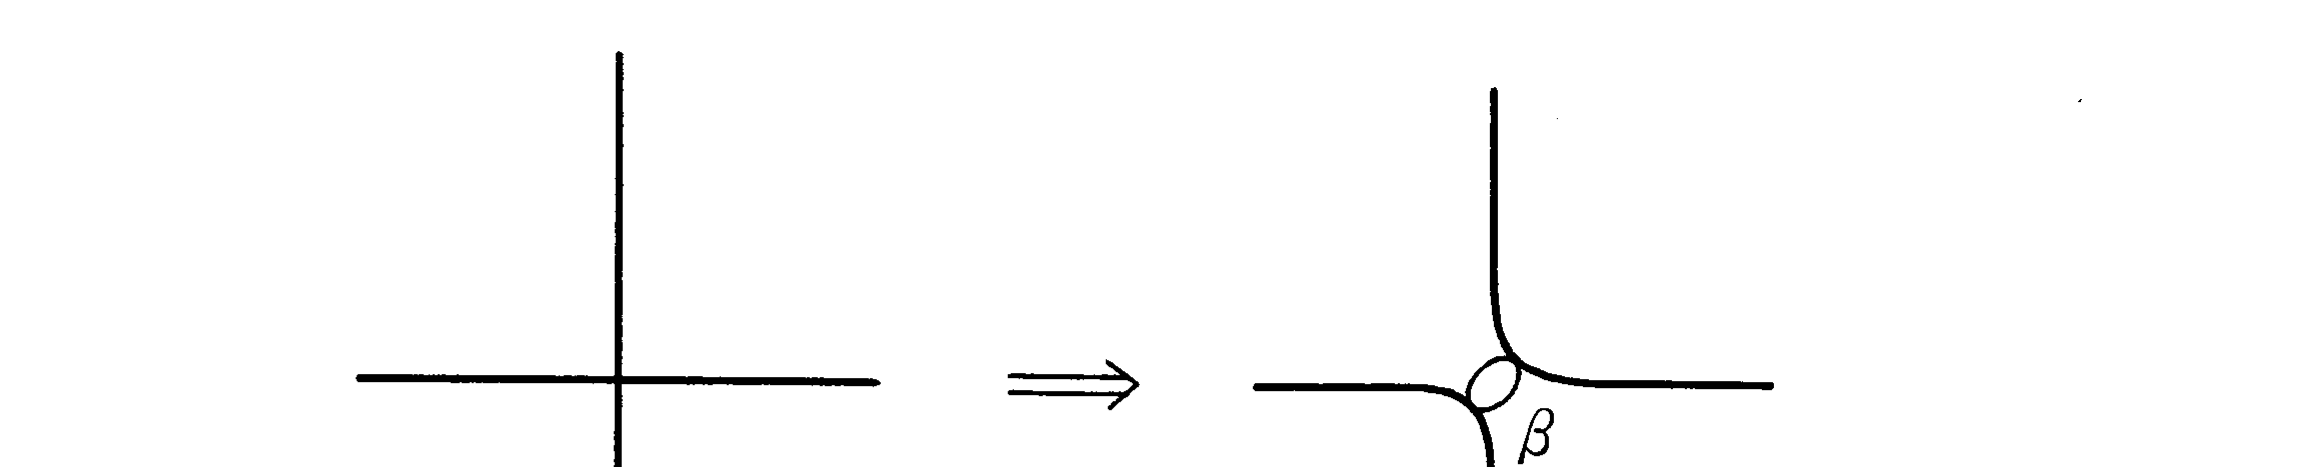
\includegraphics[width=0.72\textwidth]{figures/fig6.23.png}
  \figtitle{6.23}{消没圈（原书 p.361）}
\end{figure}

满足 (6.77) 的拉格朗日手术，可按与引理 4.145 的证明同样的方法构成，且其中出现的函数 $f_\epsilon$ 的 $\epsilon$ 的符号有正、负 2 种。取哪一种，下面叙述。

先考虑 $A$ 为单位矩阵的情形。此时连同 $L_{pt},L_{st},L_{pol}$ 在内，$T^4=\C^2/\Z[\sqrt{-1}]^2$ 是下图 6.24 中图形两张复制品的直积。此时，2 种取法由实部 $L\cap\R^2/\Z^2$ 成为图 6.25 的 (a)、(b) 中哪一个而决定。这里选取成为 (a) 的那一个。

\begin{figure}[htbp]
  \centering
  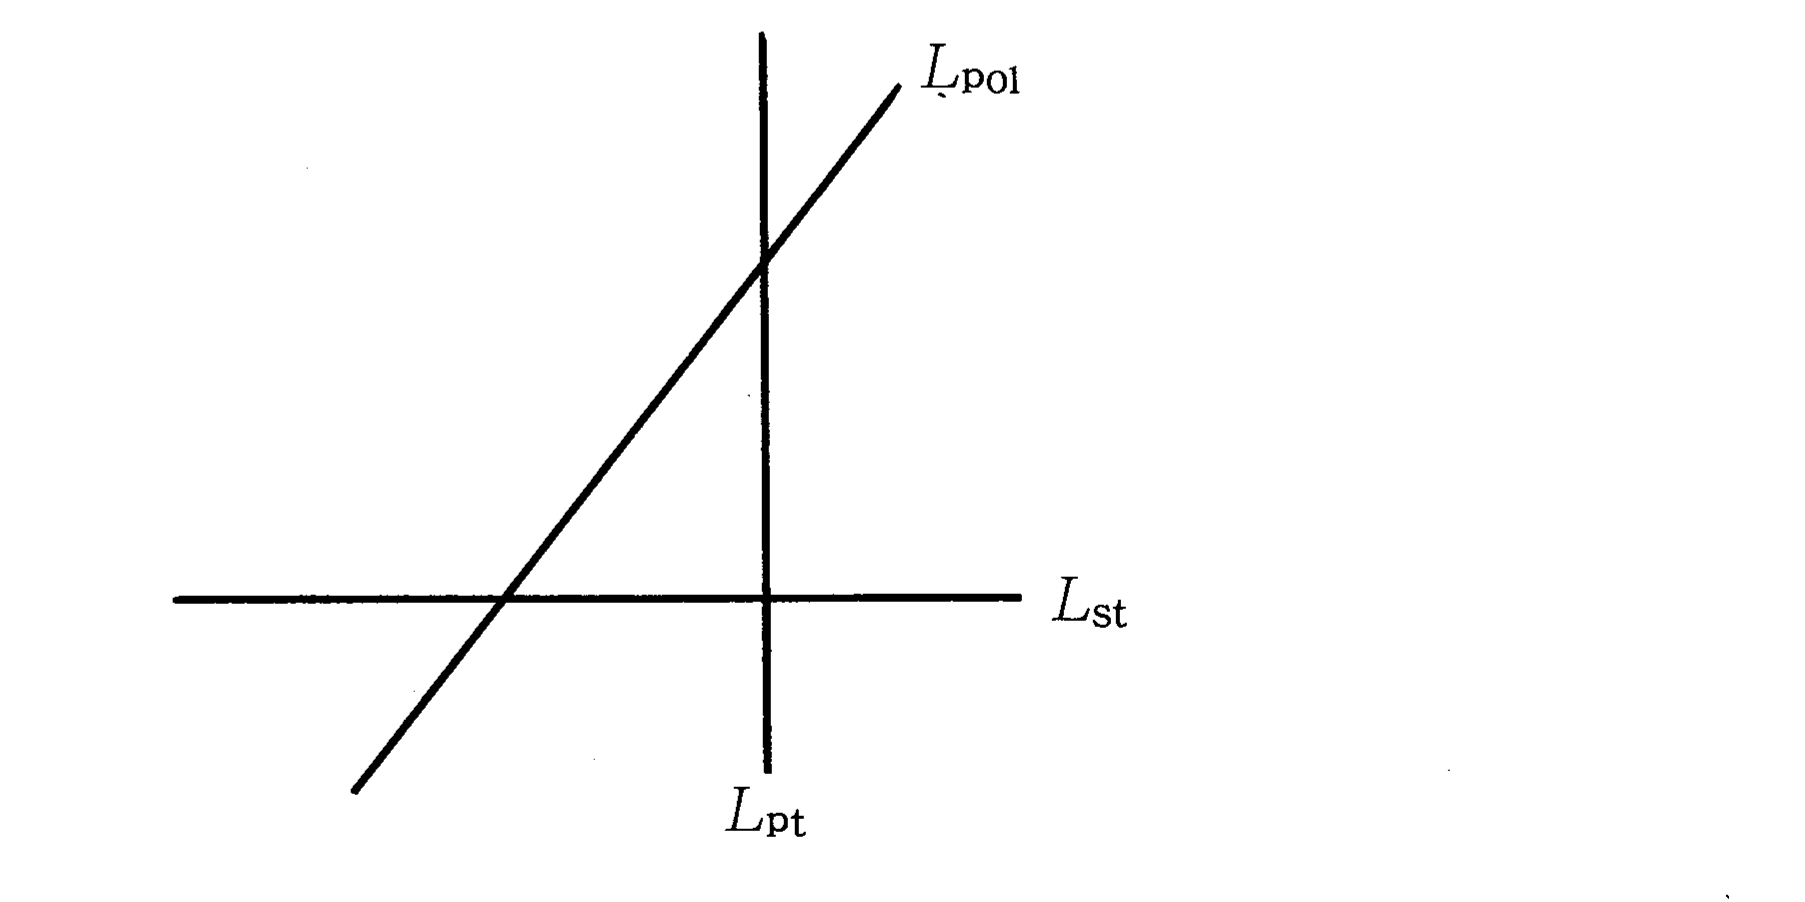
\includegraphics[width=0.52\textwidth]{figures/fig6.24.png}
  \figtitle{6.24}{（原书 p.361）}
\end{figure}

一般情形，则连续形变 $A$，并随之移动拉格朗日子流形使 (6.77) 成立，归结到 $A$ 为单位矩阵的情形，以此决定取法。

由 (6.77)，假定 5.100 成立，从而由定理 5.102，定义 Floer 上同调。

% [原文 p.362]
\begin{figure}[htbp]
  \centering
  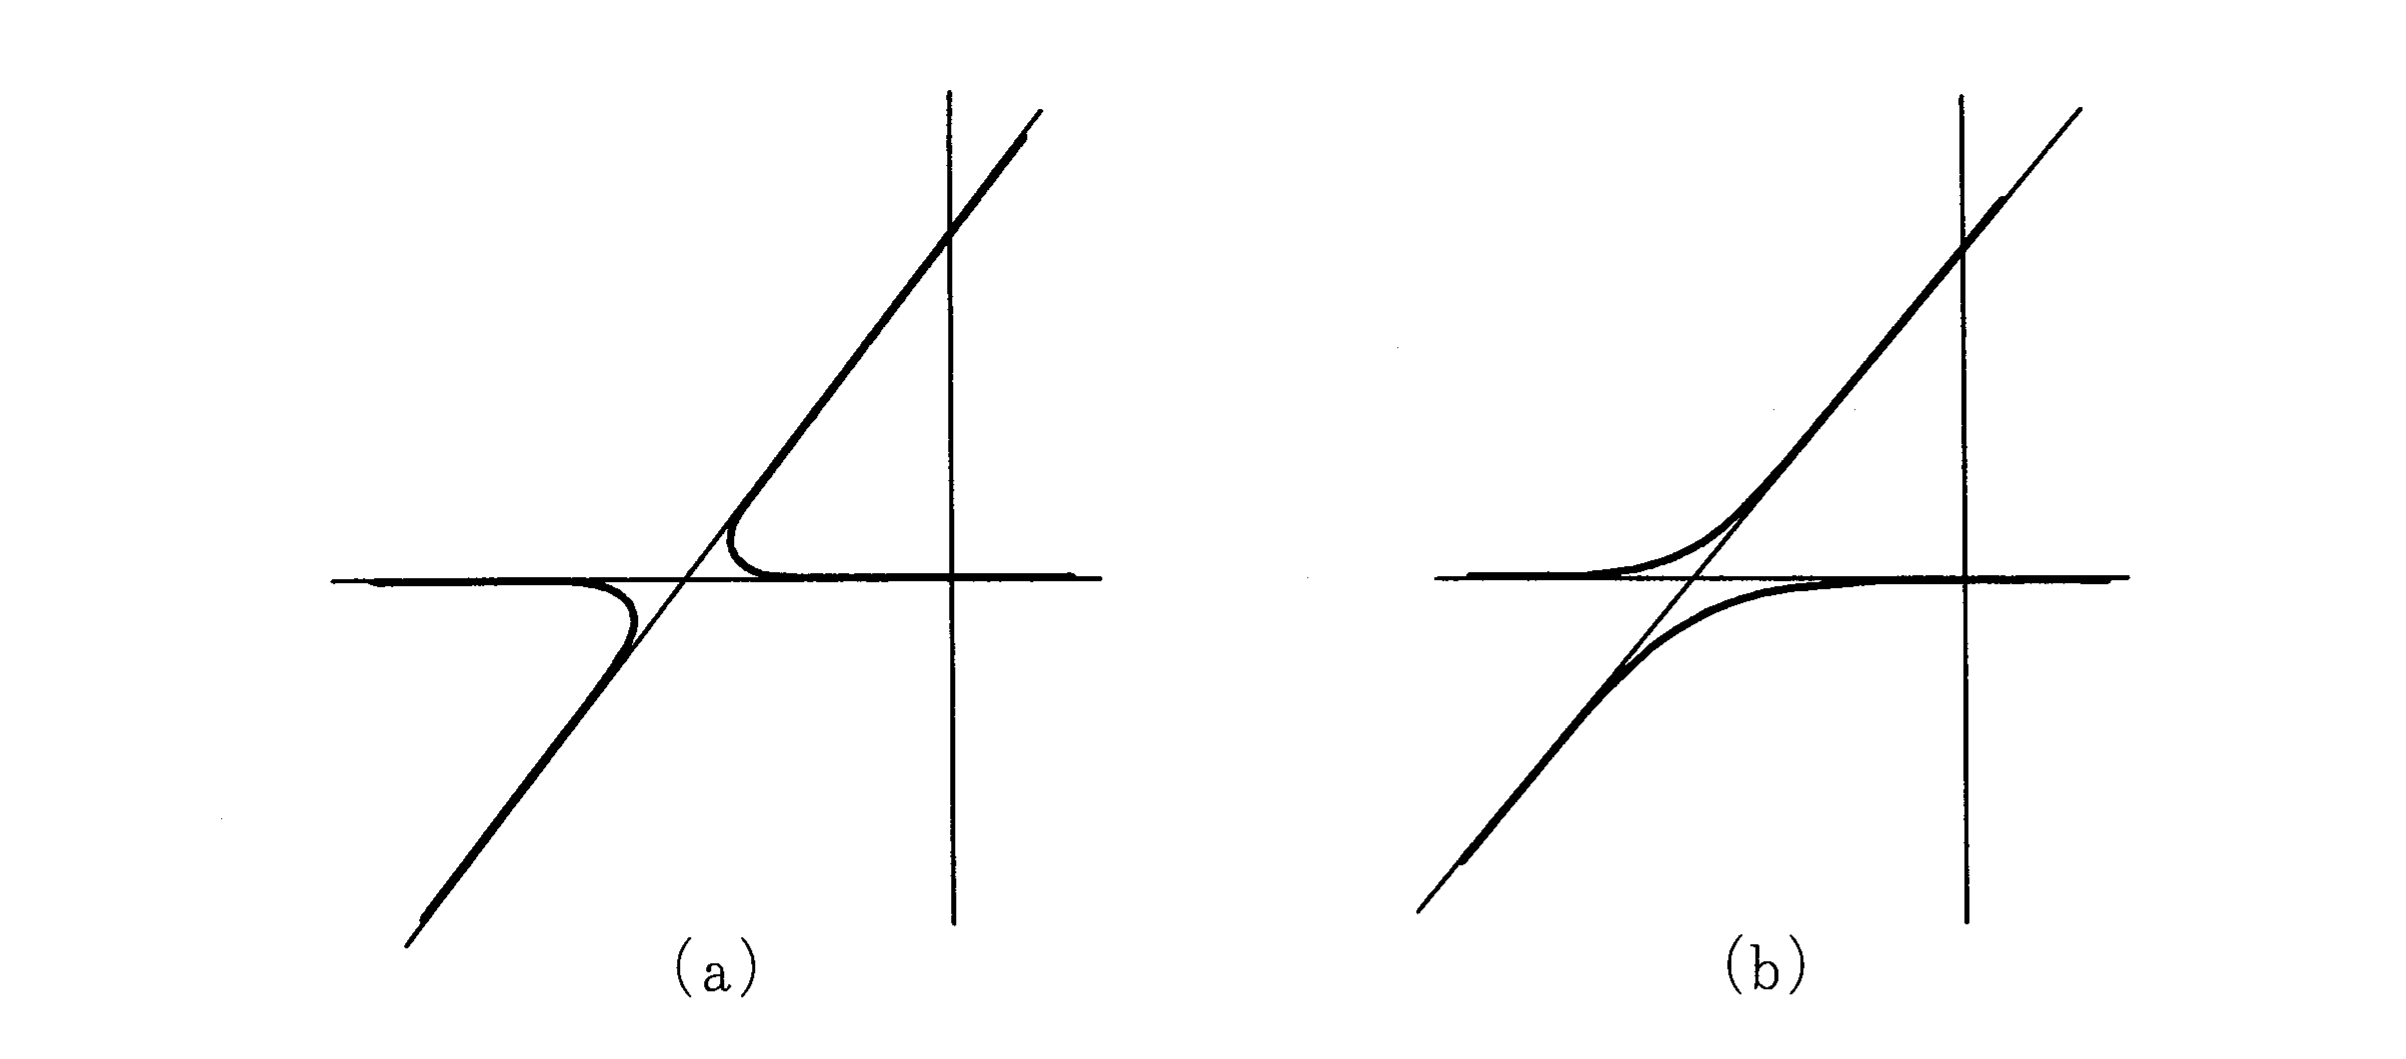
\includegraphics[width=0.80\textwidth]{figures/fig6.25.png}
  \figtitle{6.25}{与实部的交（原书 p.362）}
\end{figure}

开始计算 Floer 上同调。$L\cap L_{pt}(v)$ 由 2 点 $p,q$ 组成。这两个点的 Maslov–Viterbo 指数之差为 1。因此，确定边界算子 $\delta$ 的矩阵元素 $\langle\delta[p],[q]\rangle$ 是要点。（$\langle\delta[q],[p]\rangle$ 为 0。）

\begin{theorem}{6.240}
  $\langle\delta[p],[q]\rangle$ 是 theta 函数在 $(v,\alpha)$ 处的值。
\end{theorem}

是哪一个 theta 函数，后面再说。（有 $\nabla^\alpha$ 时的边界算子的定义也后述。）

\begin{proof}
  以 $\mathfrak{h}$ 表示上半平面。必须数出满足
  \begin{equation}
    \varphi(0)=p,\quad \varphi(\infty)=q,\quad \varphi(\R_+)\subset L_{pt}(v),\quad \varphi(\R_-)\subset L \tag{6.78}
  \end{equation}
  的伪全纯映射 $\varphi:\mathfrak{h}\to T^4$。（准确地说是数出按 $\mathfrak{h}$ 的自同构 $z\mapsto rz$（$r\in\R_+$）同一化后的等价类个数。）把这个问题归结为伪全纯三角形的问题，是第 1 阶段。考虑满足
  \begin{align}
    \varphi(0)&=p,\quad \varphi(\infty)=q,\quad \varphi(-1)=0,\notag\\
    \varphi(\R_+)&\subset L_{pt}(v),\quad \varphi([-1,0])\subset L_{st},\quad \varphi((-\infty,-1])\in L_{pol} \tag{6.79}
  \end{align}
  的伪全纯映射 $\varphi:\mathfrak{h}\to T^4$。（$\{0\}=L_{st}\cap L_{pol}$。）
\end{proof}
% [Tutor Note: 定理 6.240 的证明在此处尚未结束：原书从这一段起接着数伪全纯圆盘，并在 p.363 以引理 6.242、6.243 继续（属下一块）。本块的 ■ 只表示本页段落收束，不是论证的终点。]

\begin{proposition}{6.241}
  满足 (6.78) 的伪全纯圆盘的 $\R_+$ 作用的等价类，与满足 (6.79) 的伪全纯三角形一一对应。
\end{proposition}

证明本书省略（在 [122] 中）。它看上去正确，可从下图 6.27 看出。

其次，来研究满足 (6.79) 的伪全纯三角形。

% CHUNK ch06e DONE
